% Font options: 10pm, 11pt, 12pt
% Align headings left instead of center: nocenter
\documentclass[xcolor=x11names,compress]{beamer}\usepackage[]{graphicx}\usepackage[]{color}
%% maxwidth is the original width if it is less than linewidth
%% otherwise use linewidth (to make sure the graphics do not exceed the margin)
\makeatletter
\def\maxwidth{ %
  \ifdim\Gin@nat@width>\linewidth
    \linewidth
  \else
    \Gin@nat@width
  \fi
}
\makeatother

\definecolor{fgcolor}{rgb}{0.345, 0.345, 0.345}
\newcommand{\hlnum}[1]{\textcolor[rgb]{0.686,0.059,0.569}{#1}}%
\newcommand{\hlstr}[1]{\textcolor[rgb]{0.192,0.494,0.8}{#1}}%
\newcommand{\hlcom}[1]{\textcolor[rgb]{0.678,0.584,0.686}{\textit{#1}}}%
\newcommand{\hlopt}[1]{\textcolor[rgb]{0,0,0}{#1}}%
\newcommand{\hlstd}[1]{\textcolor[rgb]{0.345,0.345,0.345}{#1}}%
\newcommand{\hlkwa}[1]{\textcolor[rgb]{0.161,0.373,0.58}{\textbf{#1}}}%
\newcommand{\hlkwb}[1]{\textcolor[rgb]{0.69,0.353,0.396}{#1}}%
\newcommand{\hlkwc}[1]{\textcolor[rgb]{0.333,0.667,0.333}{#1}}%
\newcommand{\hlkwd}[1]{\textcolor[rgb]{0.737,0.353,0.396}{\textbf{#1}}}%
\let\hlipl\hlkwb

\usepackage{framed}
\makeatletter
\newenvironment{kframe}{%
 \def\at@end@of@kframe{}%
 \ifinner\ifhmode%
  \def\at@end@of@kframe{\end{minipage}}%
  \begin{minipage}{\columnwidth}%
 \fi\fi%
 \def\FrameCommand##1{\hskip\@totalleftmargin \hskip-\fboxsep
 \colorbox{shadecolor}{##1}\hskip-\fboxsep
     % There is no \\@totalrightmargin, so:
     \hskip-\linewidth \hskip-\@totalleftmargin \hskip\columnwidth}%
 \MakeFramed {\advance\hsize-\width
   \@totalleftmargin\z@ \linewidth\hsize
   \@setminipage}}%
 {\par\unskip\endMakeFramed%
 \at@end@of@kframe}
\makeatother

\definecolor{shadecolor}{rgb}{.97, .97, .97}
\definecolor{messagecolor}{rgb}{0, 0, 0}
\definecolor{warningcolor}{rgb}{1, 0, 1}
\definecolor{errorcolor}{rgb}{1, 0, 0}
\newenvironment{knitrout}{}{} % an empty environment to be redefined in TeX

\usepackage{alltt}
%\documentclass[xcolor=x11names,compress,handout]{beamer}
\usepackage[]{graphicx}
\usepackage[]{color}
\usepackage{booktabs}
\usepackage{hyperref}
\usepackage{tikz}
\usepackage{multirow}
\usepackage{dcolumn}
\usepackage{bigstrut}
\usepackage{amsmath} 
\usepackage{xcolor,colortbl}
\usepackage{amssymb}
%\newcommand{\done}{\cellcolor{teal}#1}

%% Beamer Layout %%%%%%%%%%%%%%%%%%%%%%%%%%%%%%%%%%
\useoutertheme[subsection=false,shadow]{miniframes}
\useinnertheme{default}
\usefonttheme{serif}
\usepackage{Arev}
\usepackage{pdfpages}

\setbeamerfont{title like}{shape=\scshape}
\setbeamerfont{frametitle}{shape=\scshape, size=\normalsize}

\definecolor{dkblue}{RGB}{0,0,102}

\setbeamercolor*{lower separation line head}{bg=dkblue} 
\setbeamercolor*{normal text}{fg=black,bg=white} 
\setbeamercolor*{alerted text}{fg=red} 
\setbeamercolor*{example text}{fg=black} 
\setbeamercolor*{structure}{fg=black} 
 
\setbeamercolor*{palette tertiary}{fg=black,bg=black!10} 
\setbeamercolor*{palette quaternary}{fg=black,bg=black!10} 

\renewcommand{\(}{\begin{columns}}
\renewcommand{\)}{\end{columns}}
\newcommand{\<}[1]{\begin{column}{#1}}
\renewcommand{\>}{\end{column}}

\AtBeginSection{\frame{\sectionpage}}
\usepackage{xcolor}
\hypersetup{
    colorlinks,
    linkcolor={red!50!black},
    citecolor={blue!50!black},
    urlcolor={blue!80!black}
}

\setbeamertemplate{navigation symbols}{} 
\setbeamertemplate{footline}[frame number]
\setbeamertemplate{caption}{\raggedright\insertcaption\par}

\setbeamersize{text margin left=5pt,text margin right=5pt}

%%%%%%%%%%%%%%%%%%%%%%%%%%%%%%%%%%%%%%%%%%%%%%%%%%


\title{FLS 6441 - Methods III: Explanation and Causation}
\subtitle{Week 11 - Comparative Case Studies \& Process Tracing}
\author{Jonathan Phillips}
\date{June 2019}
\IfFileExists{upquote.sty}{\usepackage{upquote}}{}
\begin{document}




\frame{\titlepage}

\begin{frame}
\frametitle{Classification of Research Designs}
\footnotesize
\begin{table}[htbp]
  \centering
  \scalebox{0.7}{
    \begin{tabular}{|p{2.2cm}|p{5cm}|c|c|}
    \hline
          &       & \multicolumn{1}{p{2.4cm}|}{\textbf{Independence of Treatment Assignment}} & \multicolumn{1}{p{3cm}|}{\textbf{Researcher Controls Treatment Assignment?}} \bigstrut\\
    \hline
    \multicolumn{1}{|p{2.9cm}|}{\multirow{2}[4]{2.9cm}{\textbf{Controlled Experiments}}} & Field Experiments & \checkmark      & \checkmark  \bigstrut\\
\cline{2-4}          & Survey and Lab Experiments &  \checkmark     & \checkmark \bigstrut\\
    \hline
          &       &       &  \bigstrut\\
    \hline
    \multicolumn{1}{|p{2.9cm}|}{\multirow{3}[6]{2.9cm}{\textbf{Natural Experiments}}} & Natural Experiments &  \checkmark     &  \bigstrut\\
\cline{2-4}          & Instrumental Variables & \checkmark      &  \bigstrut\\
\cline{2-4}          & Discontinuities & \checkmark      &  \bigstrut\\
    \hline
          &       &       &  \bigstrut\\
    \hline
    \multicolumn{1}{|p{2.9cm}|}{\multirow{4}[8]{2.9cm}{\textbf{Observational Studies}}} & Difference-in-Differences &       &  \bigstrut\\
\cline{2-4}          & Controlling for Confounding &       &  \bigstrut\\
\cline{2-4}          & Matching &       &  \bigstrut\\
\cline{2-4}          & Comparative Cases and Process Tracing &       &  \bigstrut\\
    \hline
    \end{tabular}}%
  \label{tab:addlabel}%
\end{table}%
\normalsize
\end{frame}

\section{Comparative Case Studies} 

\begin{frame}
\frametitle{Comparative Case Studies}
\begin{itemize}
\item Necessary when there are few measurable cases of our treatment/outcome
\pause
\item \textbf{Exactly} the same causal inference logic as Large-N
\pause
\item We need counterfactuals to estimate treatment effects: \textbf{Comparative} Cases
\pause
\item Even if we can 'observe' the causal process, we can easily make mistakes
\pause
\item The aim is to go beyond description
\end{itemize}
\end{frame}

\begin{frame}
\frametitle{Comparative Case Studies}
\begin{itemize}
\item Why can't we achieve causal inference from single case studies?
\pause
\item If we truly have only one 'treated' observation, we \textit{cannot} know what would have happened in the absence of treatment
\pause
\item These case studies can help \textit{generate} hypotheses...
\pause
\item And they can maybe reject or weaken a theory...
\pause
\item But they cannot \textbf{confirm} a theory
\pause
\item We need variation in the dependent variable if we are to explain it
\pause
\item Common error: "research that tries to explain the outbreak of war with studies only of wars" (KKV)
\end{itemize}
\end{frame}

\begin{frame}
\frametitle{Comparative Case Studies}
\begin{itemize}
\item Similarities with Large-N:
\pause
\begin{itemize}
\item Same challenges to inference: confounding, selection, reverse causation
\pause
\item Same assumptions required: SUTVA, Balance on all confounders
\pause
\end{itemize}
\item Differences with Large-N:
\begin{itemize}
\item Fewer comparisons: No uncertainty measure or confidence intervals. What's our standard of evidence?
\pause
\begin{itemize}
\item p-values aren't the only source of credibility (Slater and Ziblatt 2013)
\end{itemize}
\pause
\item Statistical Inference: Non-random cases, so generalization is harder
\pause
\item Harder to balance confounders: More variables than cases!
\end{itemize}
\end{itemize}
\end{frame}

\begin{frame}
\frametitle{Comparative Case Studies}
\begin{itemize}
\item In a small-N study, what causal inference technique is most useful?
\pause
\begin{itemize}
\item Diff-in-diff plausible if we have time-series data
\pause
\item IV may be possible if there is some as-if random assignment, eg. leader death from cancer
\pause
\item Or an RDD, eg. just missing out on WB loans due to GDP measure
\end{itemize}
\end{itemize}
\end{frame}

\begin{frame}
\frametitle{Comparative Case Studies}
\begin{itemize}
\item But most commonly, we are using a matching strategy:
\pause
\begin{itemize}
\item Matching to ensure balance on confounders through case selection - prune unmatched cases
\pause
\item Clearly we can't match on everything, so focus on getting balance on key confounders/alternative theories
\pause
\end{itemize}
\item \textbf{Our Large-N dataset after matching might look very similar to a comparative case study}
\end{itemize}
\end{frame}

\begin{frame}
\frametitle{Comparative Case Studies}
\begin{itemize}
\item Case Selection:
\pause
\item Don't confuse two distinct considerations in choosing cases:
\pause
\begin{enumerate}
\item Causal Inference (internal validity) - can our cases tell us with confidence that $D$ causes $Y$?
\pause
\item Population Inference (external validity) - How much can we generalize about this causal effect to a broader population?
\end{enumerate}
\item Ideally we want both: Control and representative variation
\begin{itemize}
\item Our goal is not to explain why revolution happened in Iran, but why it happens generally
\end{itemize}
\end{itemize}
\end{frame}

\begin{frame}
\frametitle{Comparative Case Studies}
\begin{itemize}
\item Case Selection:
\pause
\begin{itemize}
\item Random sampling is fine! It directly helps us generalize
\pause
\item And it helps us avoid explicit bias in causal inference
\pause
\item But:
\pause
\begin{itemize}
\item Randomization does not guarantee enough variation in the treatment and outcome in small samples
\pause
\item Randomization does not guarantee balance on confounders in small samples
\pause
\item Randomized sampling is not the same as randomized treatment
\end{itemize}
\item So even if we randomize, need to check for balance and variation
\pause
\item Probably easier to 'block' on key confounders and impose variation in treatment - purposive sampling
\end{itemize}
\end{itemize}
\end{frame}

\begin{frame}
\frametitle{Comparative Case Studies}
\begin{itemize}
\item Case Selection:
\pause
\begin{itemize}
\item \textbf{DO NOT} select cases by the value of the outcome (Geddes)
\pause
\item If we only study success cases, we don't know the counterfactual
\pause
\item The 'treatment' may also have been present in the 'control' cases
\pause
\item We want to explain interesting things, so we often pick 'extreme' cases, but the extremeness might reflect confounders, not the treatment
\pause
\item But: If we select cases explicitly for a \textit{range} of values of the outcome, that's better
\end{itemize}
\end{itemize}
\end{frame}

\begin{frame}
\frametitle{Comparative Case Studies}
\begin{itemize}
\item Case Selection:
\pause
\begin{itemize}
\item Case selection also requires properly defining our population/sample
\pause
\item We risk 'survival bias' if we only look at 'active' cases
\pause
\begin{itemize}
\item Eg. cases where 'deterrence' fails coincide with poor communication
\pause
\item But communication is also poor every second that deterrence worked!
\end{itemize}
\end{itemize}
\end{itemize}
\end{frame}

\begin{frame}
\frametitle{Comparative Case Studies}
\begin{itemize}
\item Case Selection:
\pause
\begin{itemize}
\item Achieving generalizability (population inference) depends on our cases being representative
\pause
\item If we want to compare mens and womens running speeds, \textbf{DO NOT} pick Usain Bolt and Florence Griffith-Joyner
\pause
\item Pick units with 'median' values - or a range of values - on the confounding and outcome variables
\pause
\item Do this at the same time as balancing confounders - hard!
\end{itemize}
\end{itemize}
\end{frame}

\begin{frame}
\frametitle{Comparative Case Studies}
\begin{itemize}
\item \textbf{Most similar cases:} Same covariates, different treatment value
\pause
\item BUT If there are many sets of 'most similar' paired cases, which should we pick?
\pause
\begin{itemize}
\item \textbf{Typical cases:} Most representative paired cases on covariates, eg. Levitsky and Way
\pause
\item \textbf{Diverse cases:} Covering all values of treatment and covariates, eg. Slater
\pause
\item \textbf{Extreme cases:} Highest and lowest values of treatment, eg. Lieberman
\end{itemize}
\end{itemize}
\end{frame}


\begin{frame}
\frametitle{Comparative Case Studies}
\begin{itemize}
\item Methods for alternative objectives:
\pause
\begin{itemize}
\item \textbf{Deviant cases:} If you want to disprove a theory or generate a new hypothesis
\pause
\item \textbf{Most different cases:} When searching for a hypothesis to explain $Y$
\pause
\item \textbf{Influential cases:} How sensitive is our relationship to mismeasurement of a key case?
\end{itemize}
\end{itemize}
\end{frame}


\begin{frame}
\frametitle{Comparative Case Studies}
\begin{itemize}
\item Three forms of mixed methods:
\pause
\begin{enumerate}
\item Large-N measurement supports case selection for Small-N analysis (Seawright and Gerring)
\pause
\item Small-N study to identify relationship, then tested for generalizability in Large-N sample (Lieberman)
\pause
\item Large-N analysis to show causal mechanism within-case, then generalized using comparative case studies (Ziblatt and Slater)
\end{enumerate}
\end{itemize}
\end{frame}

\begin{frame}
\frametitle{Comparative Case Studies}
\begin{itemize}
\item Strategies for increasing the number of observations:
\pause
\begin{enumerate}
\item Additional measurable implications of the causal theory
\pause
\item Subnational units
\pause
\item Time-series
\pause
\item Alternative mesaures
\end{enumerate}
\end{itemize}
\end{frame}

%Stress confounders as rival theories/explanations
%Most-diff-systems really about hyp-gen - perhaps use this to stress dif between causes of effects and effects of causes...


\section{Process Tracing} 

\begin{frame}
\frametitle{Process Tracing}
\begin{itemize}
\item Within-case analysis
\pause
\item Only a contribution if we can turn our single case into \textbf{multiple} observations - usually over time
\pause
\item Most effective when complementing large-N or comparative case study analysis
\pause
\item Theory-informed - the evidence must be useful for causal inference
\begin{itemize}
\item Evidence must support or undermine some theory
\pause
\item Particularly the causal mechanism - what connects $D$ to $Y$?
\pause
\item What observable implications are there of theory A?
\pause
\item Is the evidence consistent with theory A?
\end{itemize}
\end{itemize}
\end{frame}

\begin{frame}
\frametitle{Process Tracing}
\begin{enumerate}
\item Identify all relevant theories to explain the outcome (Our Treatment variable and confounders)
\pause
\item Use a specific theory to identify clear implications if each theory is true
\pause
\item Gather data from the case on each observable implication
\pause
\item Compare the data to each theory
\pause
\item Can we eliminate all other theories (confounders) except our treatment?
\begin{itemize}
\item Sherlock Holmes' Method of Elimination
\end{itemize}
\end{enumerate}
\end{frame}

\begin{frame}
\frametitle{Process Tracing}
\begin{itemize}
\item We know the value of treatment and outcome for our case - and it fits our theory
\pause
\item But we don't have any counterfactual to compare against
\pause
\item The outcome could instead have been caused by a confounder
\end{itemize}
\begin{knitrout}
\definecolor{shadecolor}{rgb}{0.969, 0.969, 0.969}\color{fgcolor}
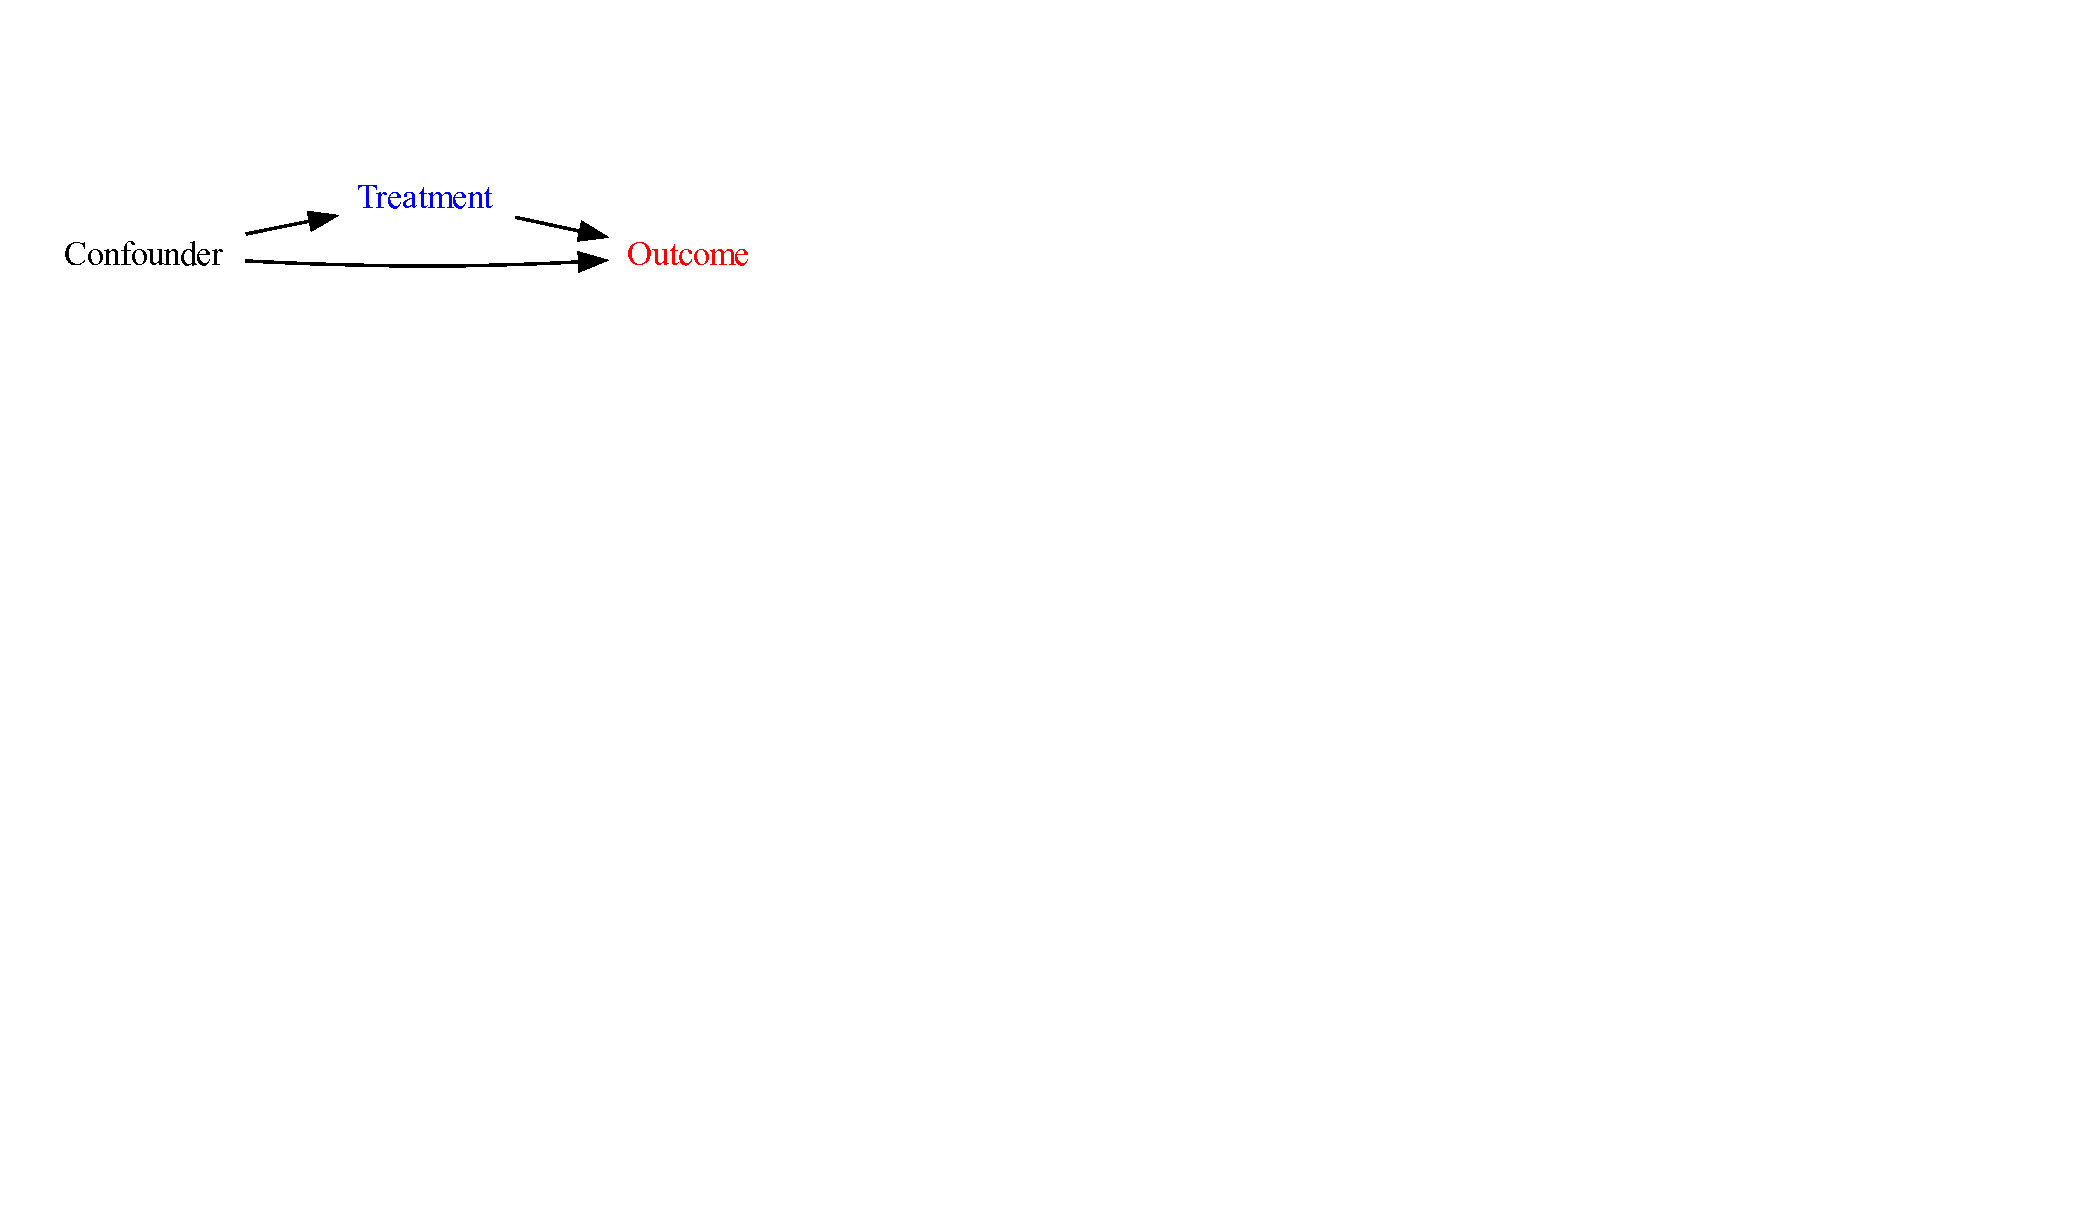
\includegraphics[width=1.8\linewidth]{figure/Dag1-1} 

\end{knitrout}
\end{frame}

\begin{frame}
\frametitle{Process Tracing}
\begin{itemize}
\item One way to support our theory is to test the mechanisms along the causal path of treatment:
\begin{itemize}
\item Evidence of M NOT occurring is proof $D$ did not have a causal effect
\item Evidence of M occurring is consistent with $D$ having a causal effect
\end{itemize}
\end{itemize}
\begin{knitrout}
\definecolor{shadecolor}{rgb}{0.969, 0.969, 0.969}\color{fgcolor}
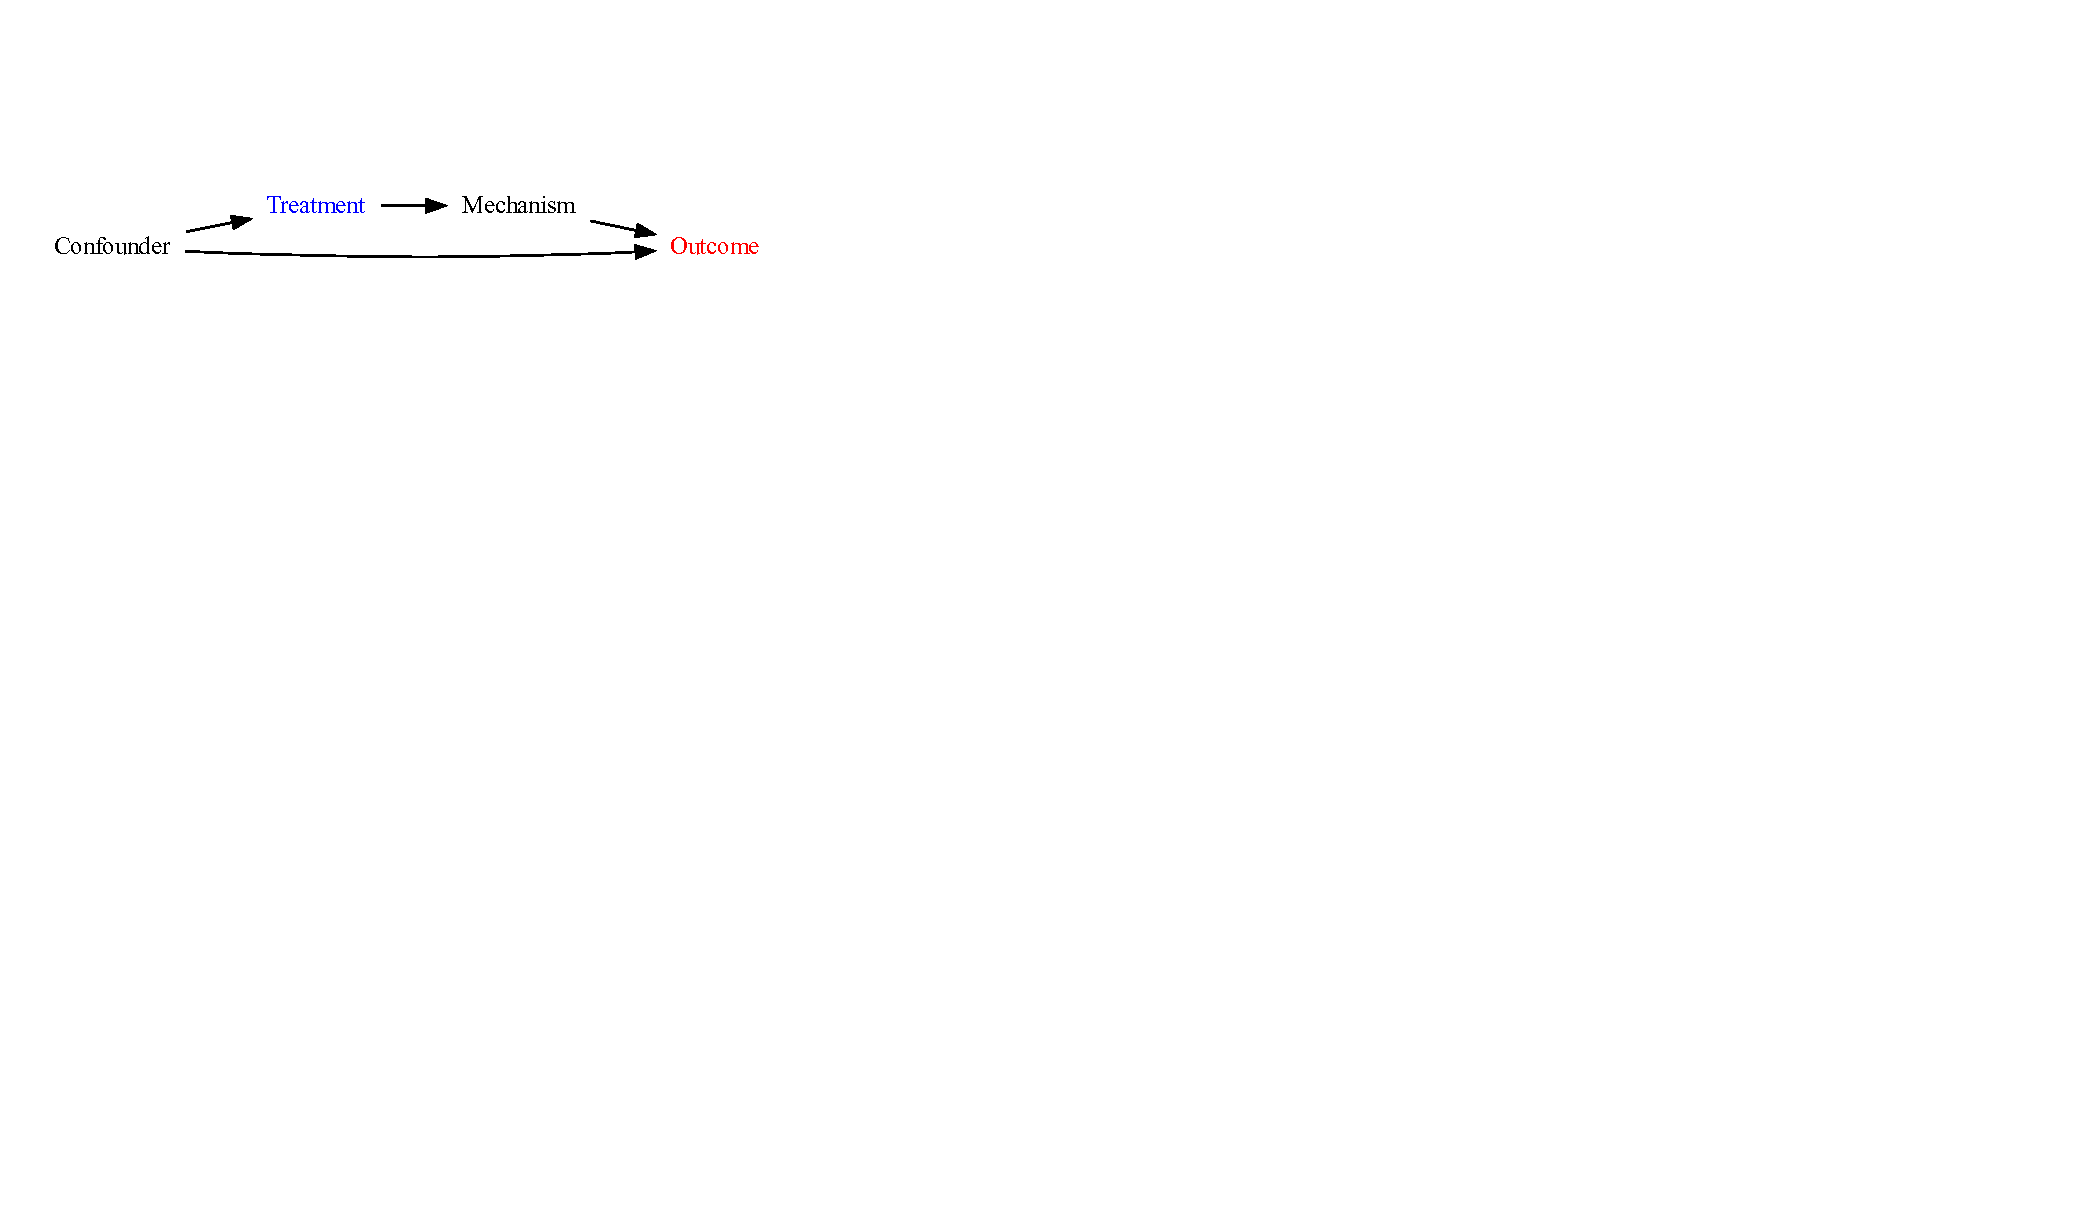
\includegraphics[width=1.8\linewidth]{figure/Dag2-1} 

\end{knitrout}
\end{frame}

\begin{frame}
\frametitle{Process Tracing}
\begin{itemize}
\item One way to support our theory is to test the mechanisms along the causal path of treatment:
\begin{itemize}
\item Evidence of M NOT occurring is proof $D$ did not have a causal effect
\item Evidence of M occurring is consistent with $D$ having a causal effect
\begin{itemize}
\item It could have been another confounder that also worked through that mechanism
\end{itemize}
\end{itemize}
\item This is a 'hoop' test
\end{itemize}
\begin{knitrout}
\definecolor{shadecolor}{rgb}{0.969, 0.969, 0.969}\color{fgcolor}
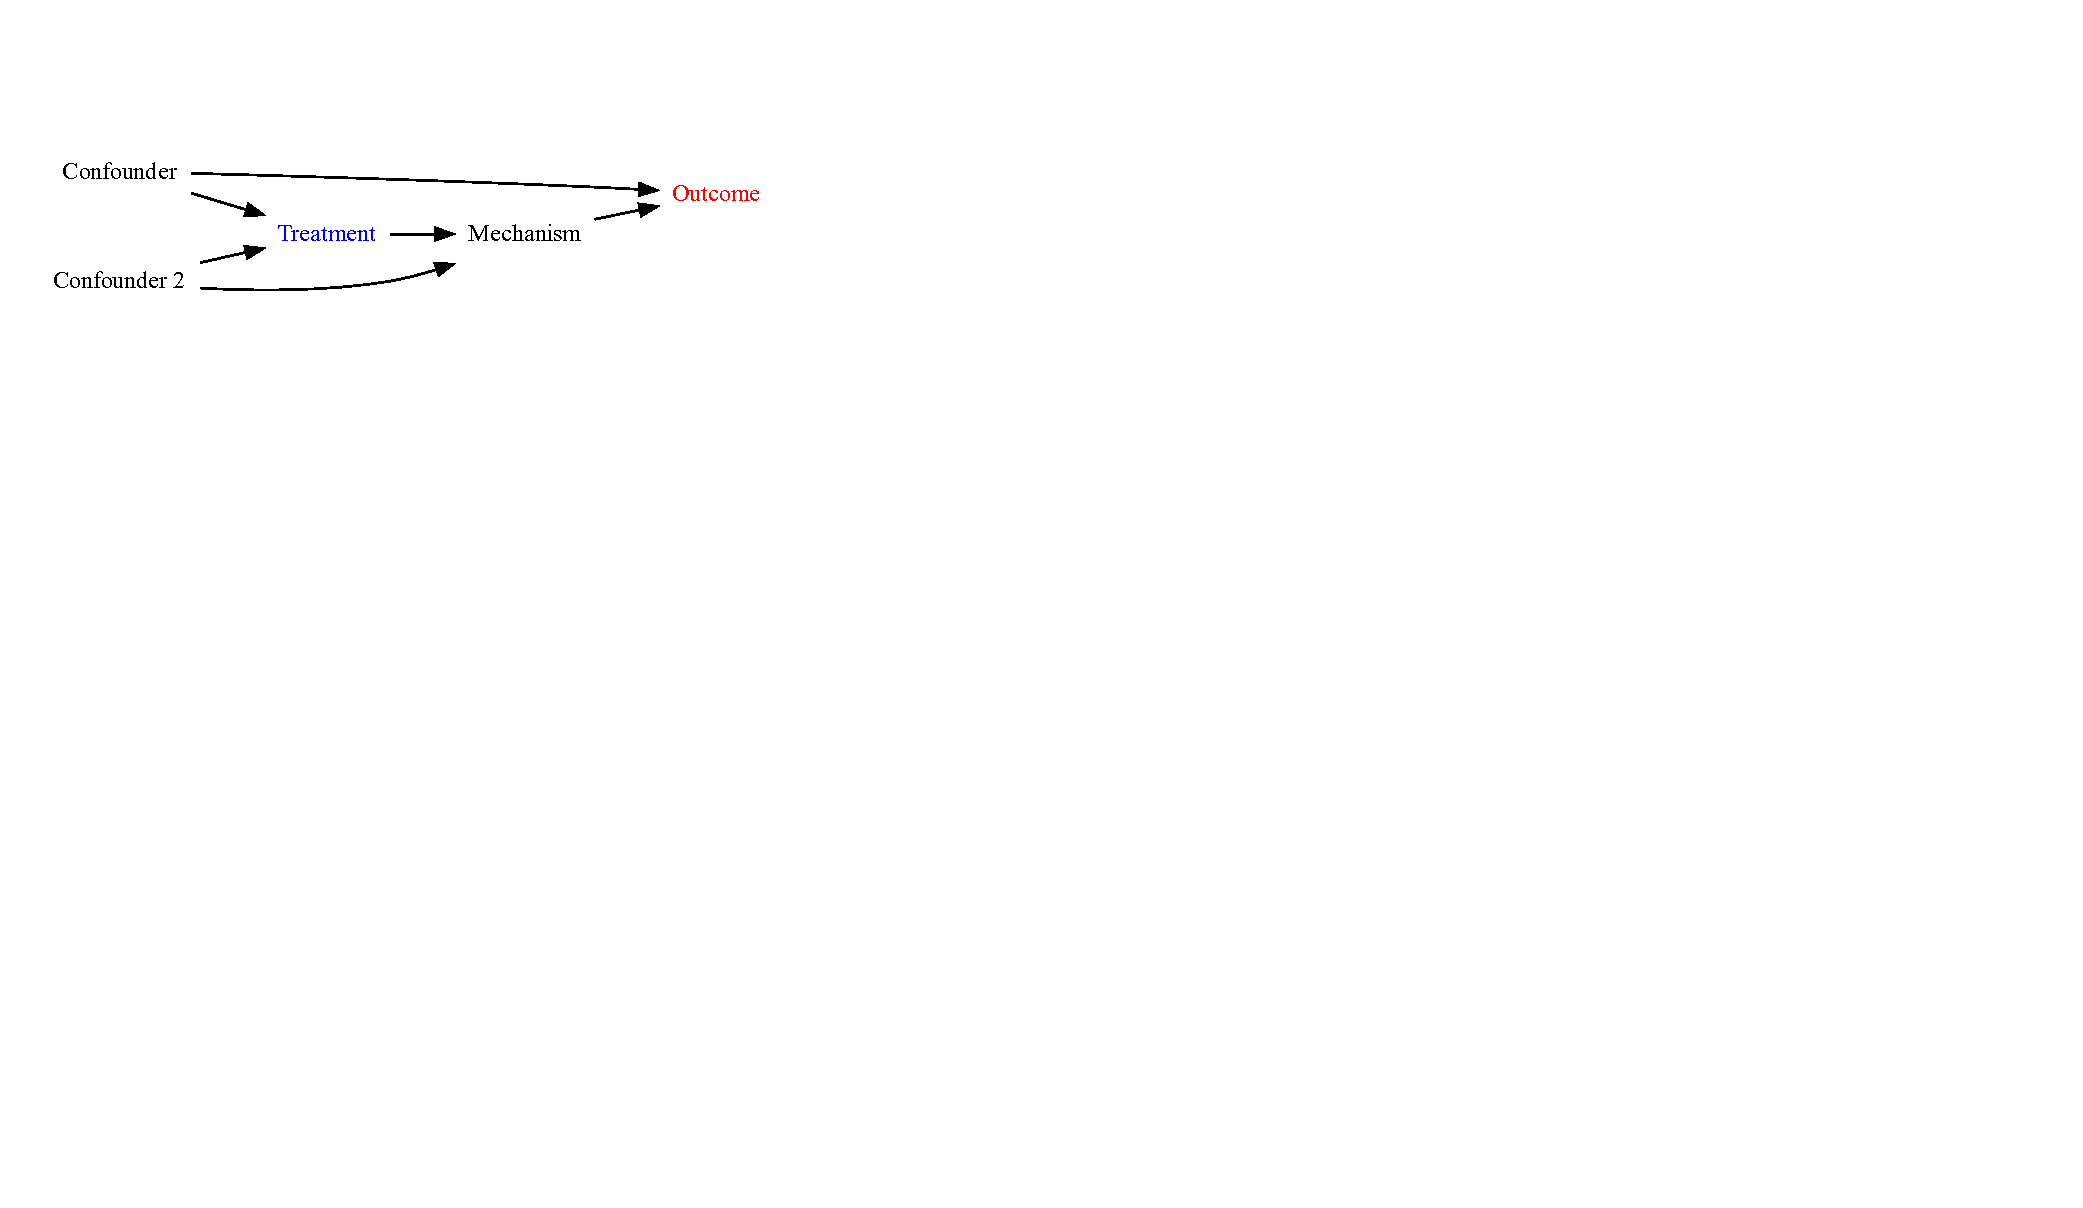
\includegraphics[width=1.8\linewidth]{figure/Dag3-1} 

\end{knitrout}
\end{frame}

\begin{frame}
\frametitle{Process Tracing}
\begin{itemize}
\item One way to support our theory is to test the mechanisms along the causal path of treatment:
\begin{itemize}
\item Evidence of M NOT occurring is proof $D$ did not have a causal effect
\item Evidence of M occurring is consistent with $D$ having a causal effect
\end{itemize}
\item If there are no other possible confounders consistent with this mechanism, this is a 'Smoking Gun' test
\end{itemize}
\begin{knitrout}
\definecolor{shadecolor}{rgb}{0.969, 0.969, 0.969}\color{fgcolor}
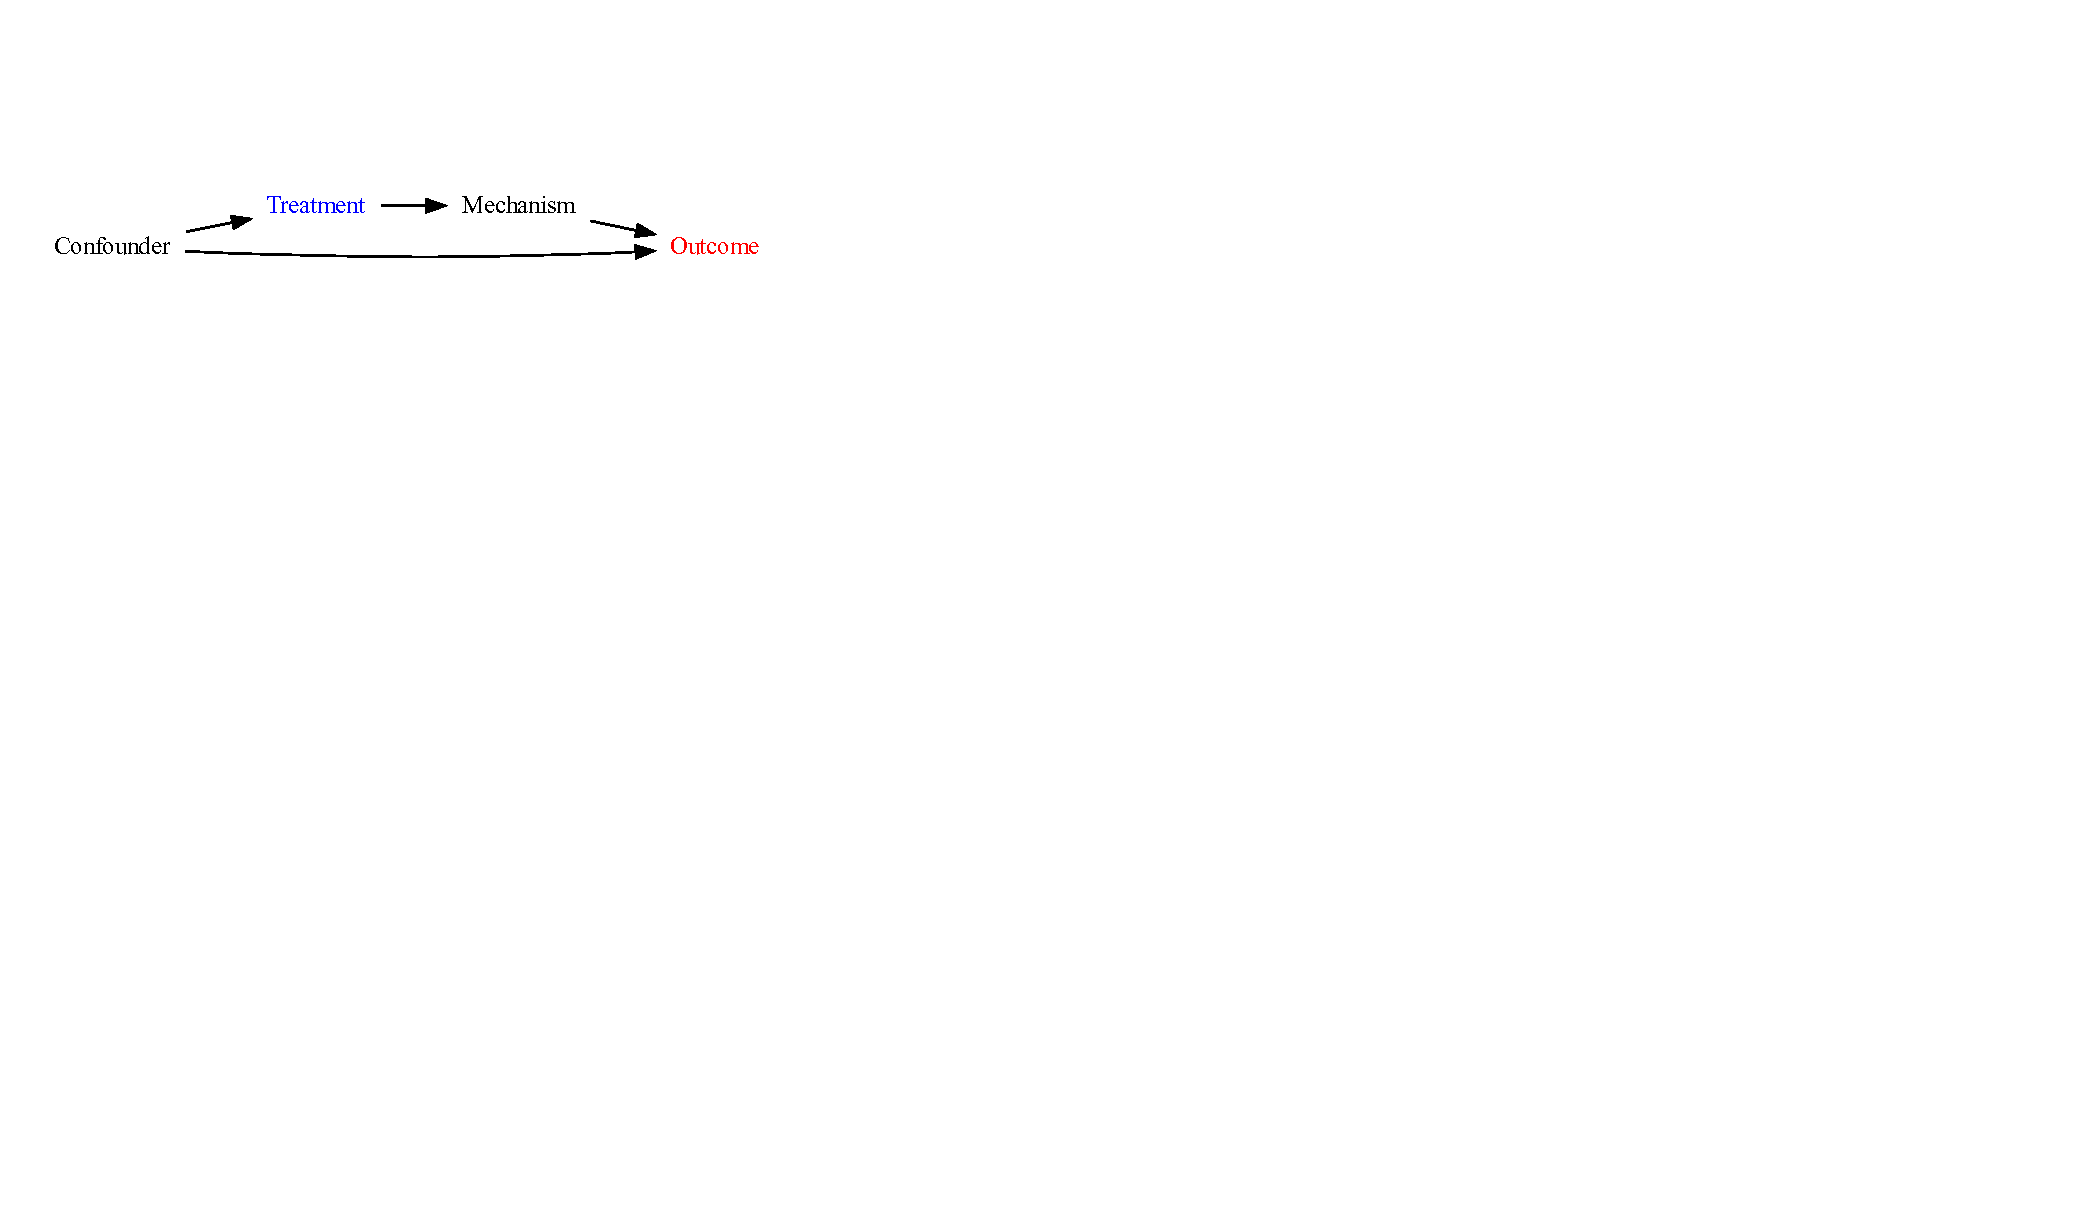
\includegraphics[width=1.8\linewidth]{figure/Dag3b-1} 

\end{knitrout}
\end{frame}


\begin{frame}
\frametitle{Process Tracing}
\begin{itemize}
\item We can also test mechanisms on the causal path of confounders:
\begin{itemize}
\item Evidence of Mechanism X NOT occurring can rule out this alternative theory
\item Evidence of Mechanism X occurring is consistent with $D$ having a causal effect, but not proof
\end{itemize}
\item This is a 'straw in the wind' test
\end{itemize}
\begin{knitrout}
\definecolor{shadecolor}{rgb}{0.969, 0.969, 0.969}\color{fgcolor}
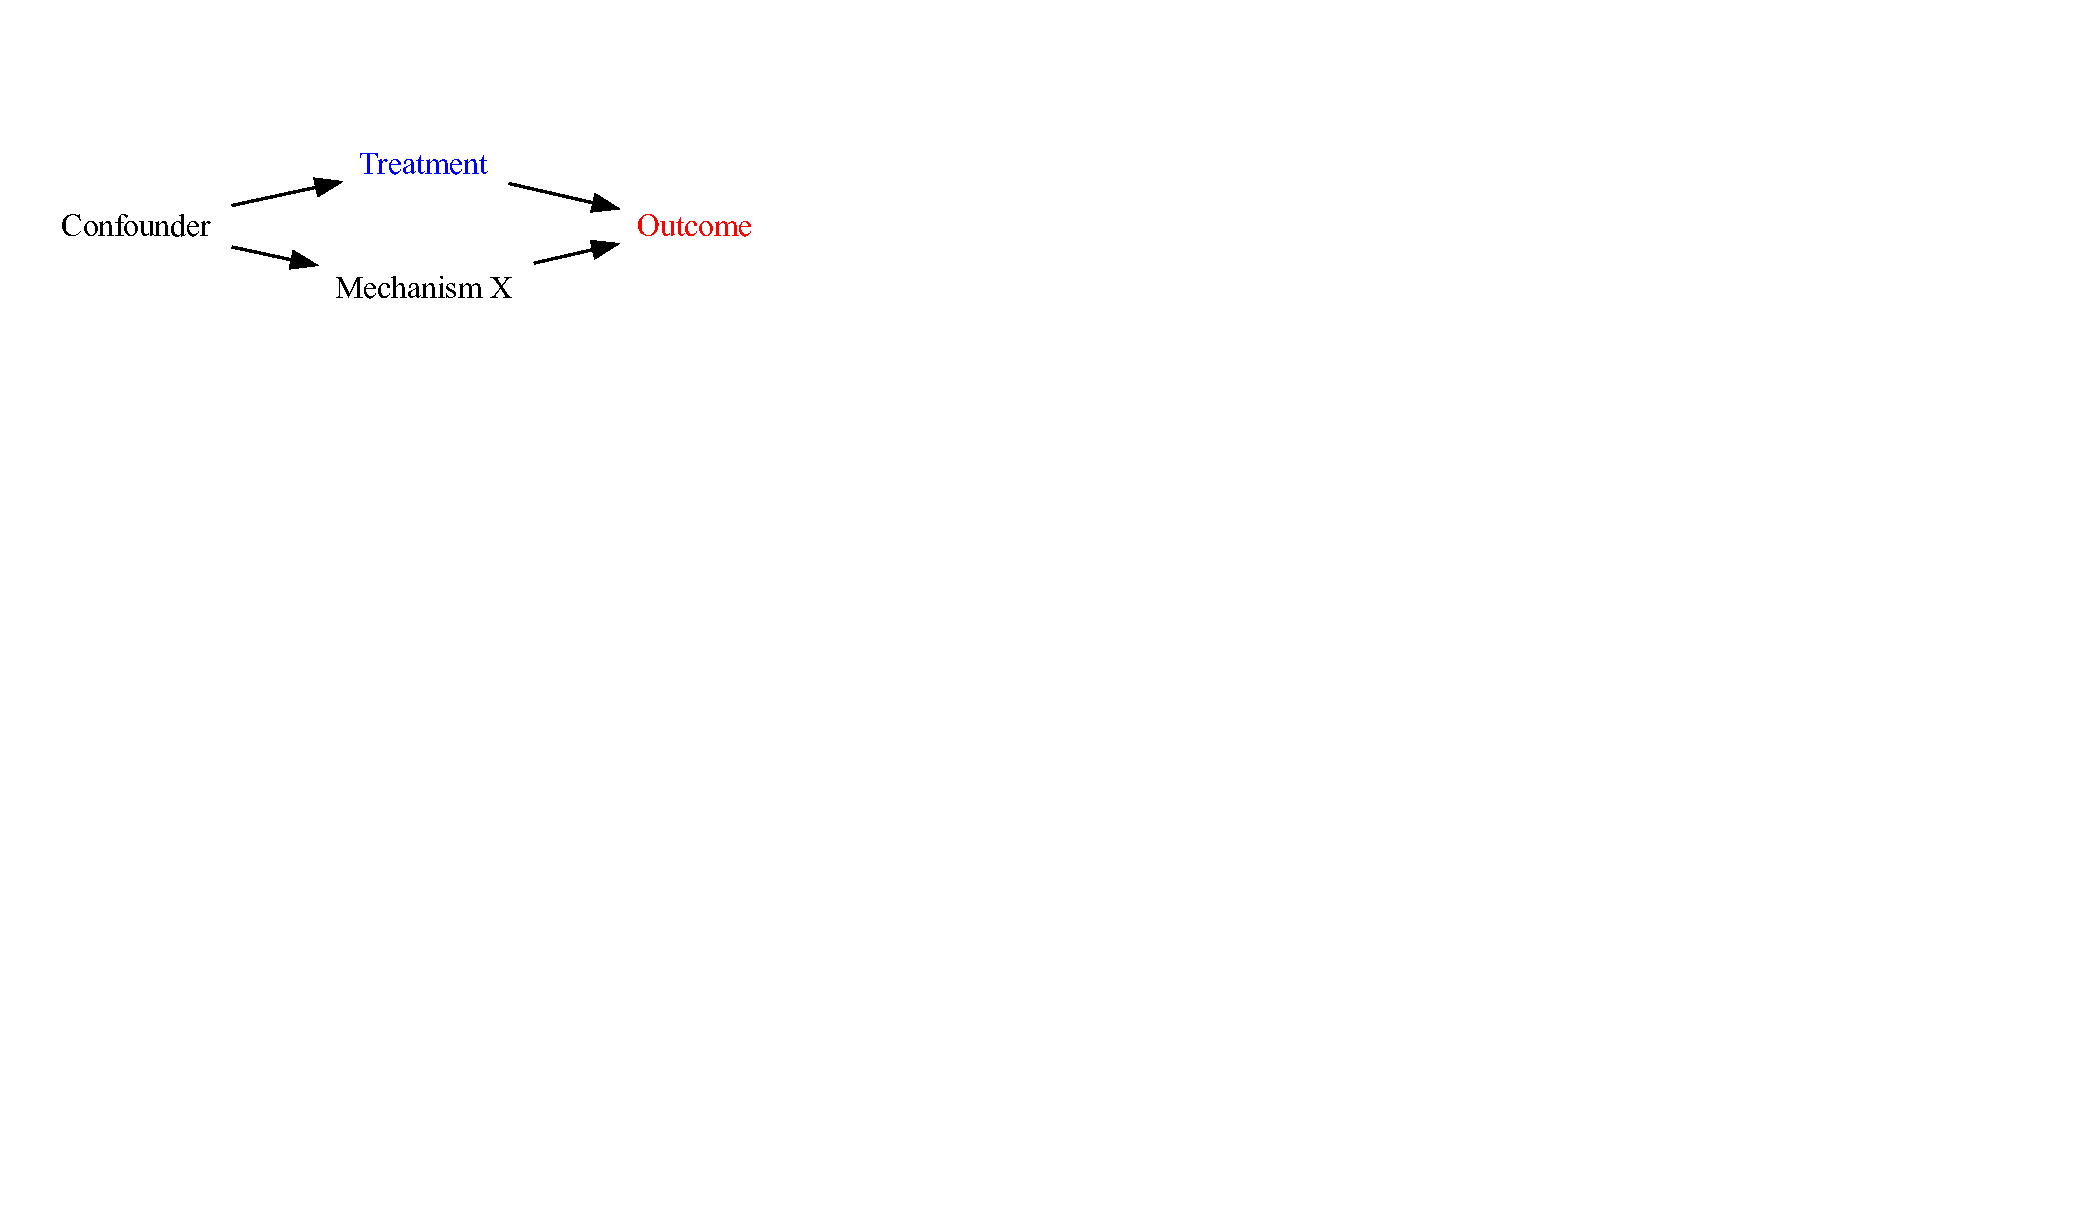
\includegraphics[width=1.8\linewidth]{figure/Dag4-1} 

\end{knitrout}
\end{frame}

\begin{frame}
\frametitle{Process Tracing}
\begin{itemize}
\item Unusually, a mechanism might explicitly separate two theories:
\begin{itemize}
\item $M=0$ if treatment is active
\item $M=1$ if the confounder is active
\end{itemize}
\item This is a 'Doubly-Decisive' test
\end{itemize}
\begin{knitrout}
\definecolor{shadecolor}{rgb}{0.969, 0.969, 0.969}\color{fgcolor}
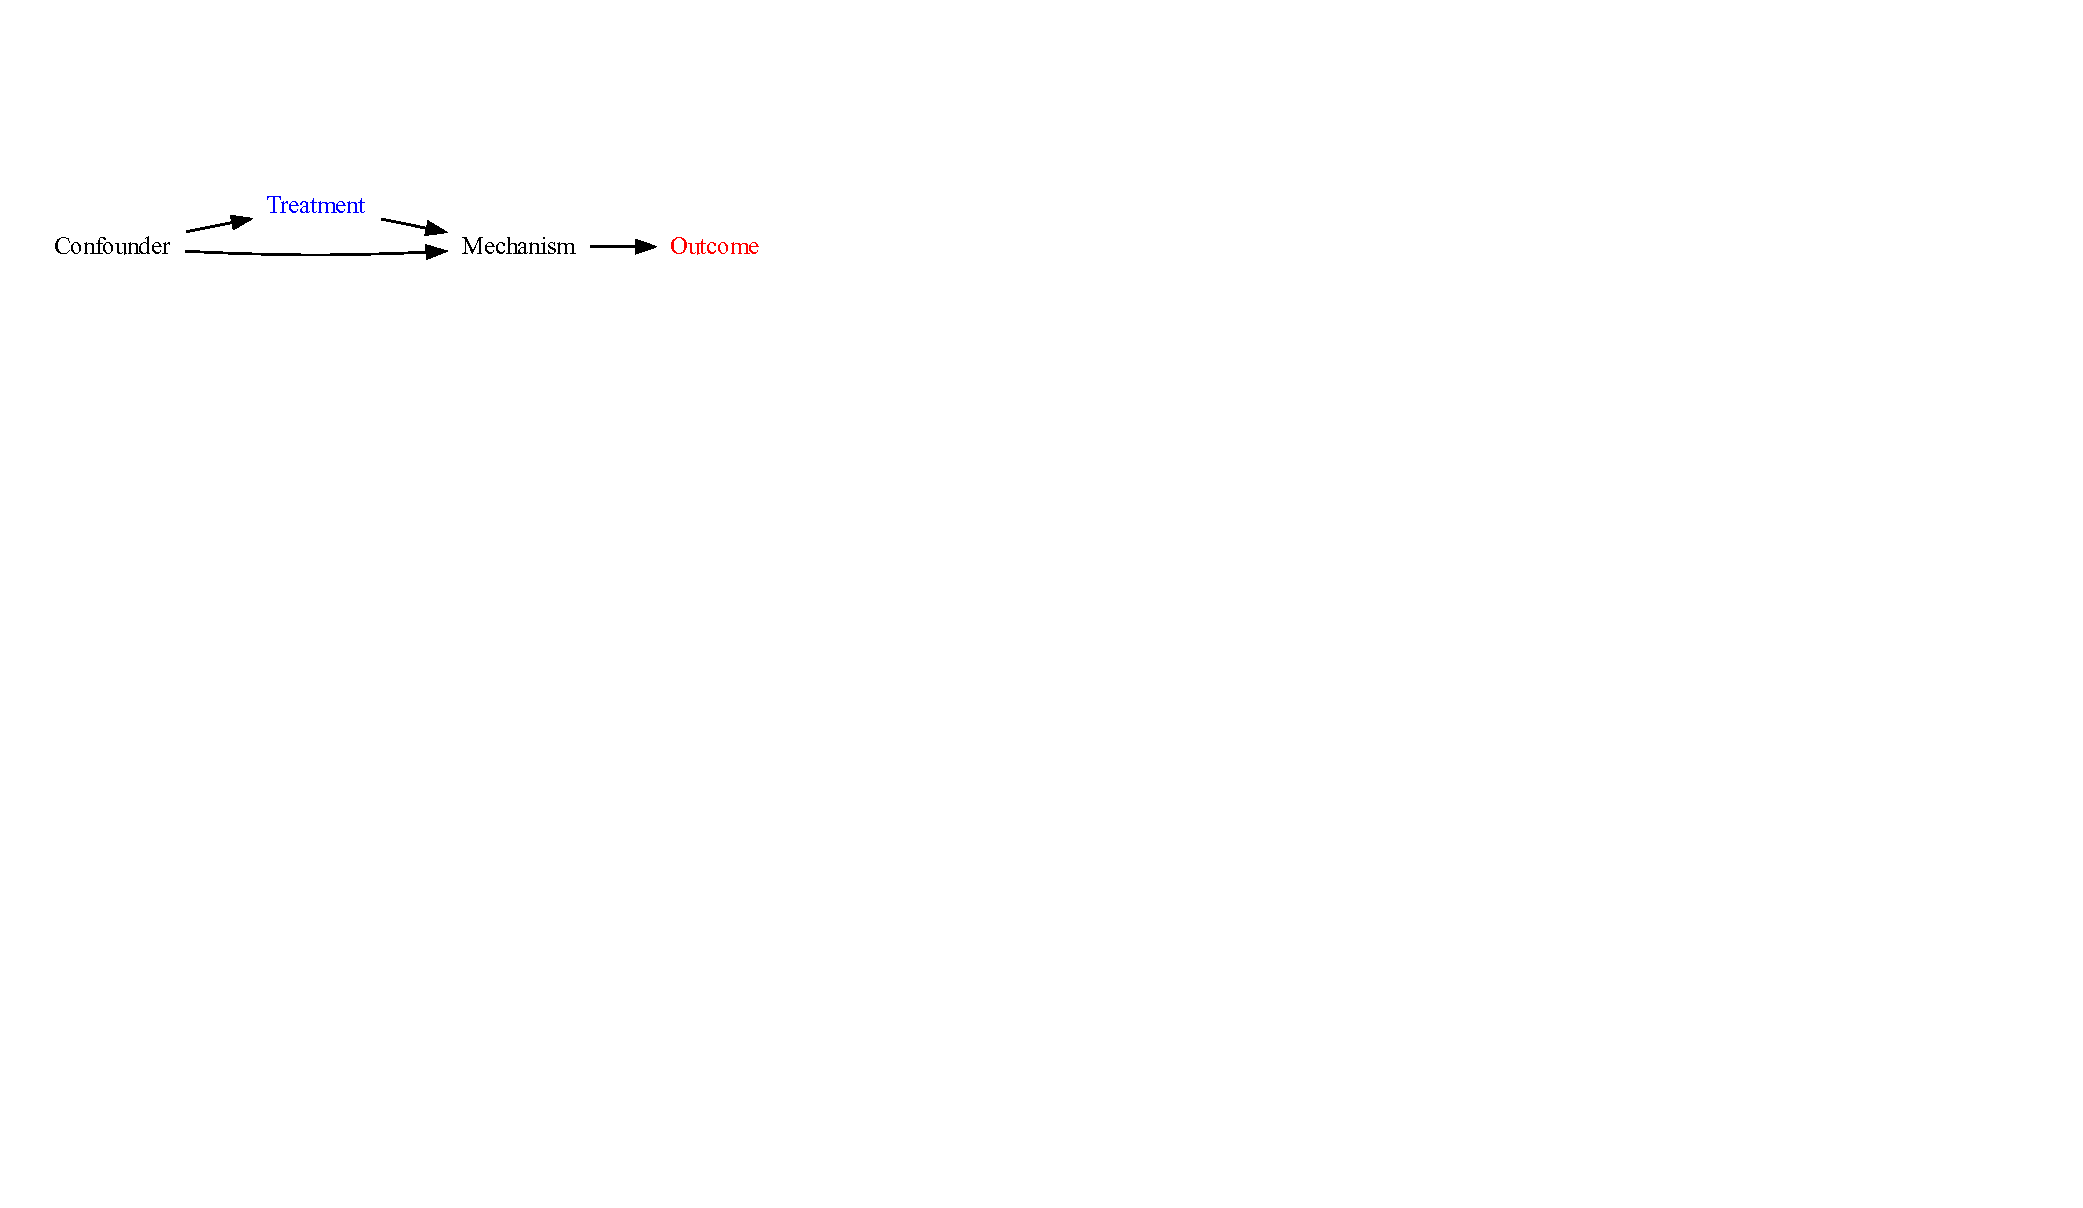
\includegraphics[width=1.8\linewidth]{figure/Dag5-1} 

\end{knitrout}
\end{frame}

\begin{frame}
\frametitle{Process Tracing}
\begin{itemize}
\item What happened to counterfactuals here?
\pause
\item We still don't know what would have happened if our case had not received the treatment
\pause
\item We're substituting assumptions/theory for a counterfactual
\pause
\begin{itemize}
\item We 'assume' that the only way our treatment could work is through the mechanism we specify
\pause
\item And we assume the only way confounding works is through the mechanism we specify
\end{itemize}
\item So everything depends on how confident we are in our theory/assumptions about mechanisms
\pause
\item Note the pattern from least to most theoretical as we require more and more prior knowledge to make causal inference: Field experiments, natural experiments, observational studies, comparative cases, process tracing
\end{itemize}
\end{frame}

\begin{frame}
\frametitle{Process Tracing}
\begin{itemize}
\item In practice, process tracing is made harder by:
\pause
\begin{itemize}
\item Imprecise, multiple or non-discriminating theory
\pause
\item Imperfect measurement and data availability
\pause
\item Subjective judgment on the weight of each piece of evidence
\end{itemize}
\end{itemize}
\end{frame}

\begin{frame}
\frametitle{Process Tracing}
\begin{itemize}
\item What are we really learning from process tracing?
\pause
\item That a treatment caused an outcome \textbf{in our specific case}
\pause
\item That is a form of causal inference - if $D$ has caused $Y$ then it must be capable of having some effect in a broader sample
\pause
\item But how representative is our case?
\pause
\item Will the same causal effect occur in other contexts?
\end{itemize}
\end{frame}

\begin{frame}
\frametitle{Process Tracing}
\begin{itemize}
\item One advantage is that we can focus on individuals' preferences, behaviour, perceptions, expectations and decisions
\pause
\item Process tracing also more useful where causation is complex - with lots of interaction effects, context-specific causation, feedback effects and multiple equilibria
\end{itemize}
\end{frame}

\begin{frame}
\frametitle{Process Tracing}
\begin{itemize}
\item Analytic Narratives
\pause
\begin{itemize}
\item Using the causal mechanisms in formal theory (game theory) to generalize from case studies
\pause
\item Iterates between the case study and the theory
\pause
\item Case study defines the players, preferences and strategy set (options) in the game theory
\pause
\item Game theory predictions are compared to the outcomes in the case study
\pause
\end{itemize}
\item The game theory then provides for causal inference - allows us to generalize a causal mechanism for how the treatment affects the outcome
\pause
\item The game might make bad predictions - that suggests this treatment/theory is wrong
pause
\item But the risk is we don't test alternative theories, we just amend our original model slightly
\end{itemize}
\end{frame}

%Causal Process Observations
%Framework relies on deterministic effects, not probabilistic ones (really means we've taken all the confounders into account)
%Can also look at 'other' auxiliary outcomes
%When to start an analysis? If theory-generating...

\begin{frame}
\frametitle{Process Tracing}
\begin{itemize}
\item Brady (2010)
\pause
\item Difference-in-differences evidence that the early announcement of a Democrat victory in Florida led to reduced Republican voting
\pause
\item Estimated 10,000 lost Republican votes
\pause
\item Is this a reasonable estimate? Process tracing goes beyond the treatment, outcome and confounder data to use evidence on the mechanisms
\pause
\item The only way the causal effect is true is if there is a causal mechanism connecting the treatment to the outcome:
\end{itemize}
\end{frame}

\begin{frame}
\frametitle{Process Tracing}
\begin{itemize}
\item Brady (2010)
\pause
\begin{itemize}
\item How long was left for the election after treatment? \pause 10 minutes
\pause
\item How many voters were \textbf{potentially influenced} \pause 4,200 voters
\pause
\item How many voters were \textbf{probably treated} \pause 560 voters
\pause
\item How many voters \textbf{likely complied with treatment} \pause 56 voters \pause \< 10,000
\end{itemize}
\end{itemize}
\end{frame}

\section{}

\begin{frame}
\frametitle{Process Tracing}
\begin{itemize}
\item Brady (2010)
\pause
\begin{itemize}
\item How long was left for the election after treatment? \pause 10 minutes
\pause
\item How many voters were \textbf{potentially influenced} \pause 4,200 voters
\pause
\item How many voters were \textbf{probably treated} \pause 560 voters
\pause
\item How many voters \textbf{likely complied with treatment} \pause 56 voters \pause \< 10,000
\end{itemize}
\end{itemize}
\end{frame}




\end{document}
